\documentclass[11pt,a4paper]{article}
\usepackage[a4paper,margin=2.6cm]{geometry}
\usepackage{iftex}
\ifPDFTeX
  \usepackage[T2A]{fontenc}
  \usepackage[utf8]{inputenc}
  \usepackage[russian]{babel}
\else
  \usepackage{fontspec}
  \usepackage{polyglossia}
  \setdefaultlanguage{russian}
  \setotherlanguage{english}
  \defaultfontfeatures{Ligatures=TeX}
  \setmainfont{Times New Roman}
  \setsansfont{Arial}
  \setmonofont{Courier New}
  \newfontfamily\cyrillicfont{Times New Roman}
  \newfontfamily\cyrillicfontsf{Arial}
  \newfontfamily\cyrillicfonttt{Courier New}
\fi
\usepackage{microtype}
\usepackage{mathtools,amssymb}
\usepackage{graphicx}
\usepackage{booktabs}
\usepackage{float}
\usepackage{caption}
\captionsetup{font=small,labelfont=bf}
\usepackage{enumitem}
\setlist{nosep,leftmargin=1.5em}
\usepackage{csquotes}
\usepackage[backend=biber,style=numeric-comp,sorting=none,maxbibnames=6]{biblatex}
\addbibresource{references_v2.bib}
\usepackage[unicode,hidelinks]{hyperref}
\setlength{\emergencystretch}{2em}

\title{Сопряжённость иерархических уровней атмосферной циркуляции\\
как региональный инвариант}
\author{Сотириади Н.}
\date{2026}

\begin{document}
\maketitle

\begin{abstract}
Иерархические уровни организации геосистем принято выделять по спектральным и фрактальным свойствам полей; вопрос о том, как измерить \emph{взаимодействие} выделенных уровней и обладает ли рисунок этого взаимодействия свойствами инварианта территории, до сих пор оставался открытым. В работе предложен компактный дескриптор такого взаимодействия --- профиль сопряжённости соседних октавных уровней~$P$, то есть пространственная ранговая корреляция карт активности уровней поля относительного вихря на изобарической поверхности 850~гПа. Материал --- реанализ ERA5 для 39 областей размером $20^\circ\times40^\circ$, покрывающих основные циркуляционные режимы; сезоны январь--март и июль--сентябрь, для двенадцати содержательно выбранных областей --- три периода 2017--2024~гг., для двадцати семи областей формальной решётки --- 2024~г. Схема исследования построена на заранее фиксируемых критериях, суррогатных нулях и подтверждении каждого утверждения на выборках, не участвовавших в его получении. Показано, что профиль образует устойчивую региональную сигнатуру ($p=0{,}001$), сохраняющуюся при смене сезона, года и фазы ЭНСО, не сводится к спектральным характеристикам уровней и к симметричным статистикам межмасштабной связи и воспроизводится в независимом реанализе MERRA-2. Ключевая проверка --- расчёт по свободному, не усваивающему наблюдений модельному эксперименту высокого разрешения: региональная география сопряжённости воспроизводится и там ($\rho=0{,}71$ при внутреннем пределе метода $0{,}93$), что снимает главное ограничение подобных работ --- невозможность отделить свойство атмосферы от свойства наблюдательной сети. Приведён каталог проверенных и отвергнутых интерпретаций, включая отвергнутую конструкцию второго дескриптора. Прикладное содержание величины на сегодняшних данных и моделях не установлено; показано, в чём именно состоит ограничение.

\smallskip
\noindent\textbf{Ключевые слова:} иерархическая организация геосистем, инварианты, масштаб, атмосферная циркуляция, реанализ, районирование, генерализация.
\end{abstract}

\section{Постановка}
\label{sec:intro}

\subsection{Инварианты организации территории}

Представление о геосистемах как об иерархически организованных образованиях, в которых процессы разных пространственно-временных уровней связаны, но не сводимы друг к другу, принадлежит к числу основополагающих в отечественной теоретической географии. В работах Ю.\,Г.~Пузаченко эта идея получила операциональное развитие: пространственно-временная иерархия геосистем рассмотрена с позиций теории колебаний \cite{Puzachenko1986}, сформирован аппарат выделения уровней организации по спектральным и фрактальным свойствам географических полей \cite{Puzachenko2004}, а поиск \emph{инвариантов динамики геосистем} --- устойчивых во времени числовых характеристик организации, различающих территории, --- поставлен как самостоятельная исследовательская программа \cite{Puzachenko2010}. Инвариант в этом понимании не есть константа природы; это воспроизводимая мера устройства территории, сохраняющая значение при смене состояния системы и потому пригодная для сравнения и районирования.

Непосредственным развитием линии стала работа А.\,Н.~Кренке с соавторами \cite{Krenke2019}, где иерархические уровни организации регионального мезоклимата выделялись по двумерным спектрам главных компонент климатических полей: степенная модель спектра играла роль фона, а отклонения от неё --- изломы наклона и субгармонические пики --- интерпретировались как проявления дискретных уровней с характерными линейными размерами. Тем самым получен ответ на вопрос, \emph{где} расположены уровни организации.

Следующий по логике вопрос --- как измерить \emph{отношение} между уровнями: насколько размещение изменчивости одного уровня предопределено соседним. Величины такого рода до сих пор не строились как самостоятельные характеристики территории и не проверялись на статус инвариантов. Настоящая работа посвящена этому вопросу применительно к атмосферной циркуляции.

\subsection{Чего не измеряют существующие подходы}

Близкие по духу инструменты развивались в трёх традициях, и каждая оставляет искомую величину за пределами рассмотрения. Каскадные и мультифрактальные описания \cite{LovejoySchertzer2013,Lovejoy2011,Kouhen2024} характеризуют распределение интенсивности \emph{вдоль} масштабного континуума, но не пространственную согласованность карт активности \emph{между} конкретными уровнями. Вейвлет-огибающие и их статистики --- коэффициент амплитудной модуляции \cite{Farge1992,Mathis2009} и систематизирующие его скаттеринг-ковариации \cite{Mallat2012,BrunaMallat2013,Cheng2024} --- измеряют факт связи уровней, но применялись как признаки для классификации, а не как климатология устройства территории; первое приложение подобной техники к геофизическим полям с целью различения режимов появилось недавно и относится к океану \cite{Skinner2025}. Наконец, литература о предсказуемости атмосферы \cite{Lorenz1969,Zhang2007,RotunnoSnyder2008,Judt2020,SelzCraig2023} отводит межмасштабному взаимодействию роль канала, по которому неопределённость мелких масштабов заражает синоптический уровень, но \emph{моделирует} силу этой связи, а не измеряет её по данным.

\subsection{Задачи}

(1)~Построить по полю относительного вихря компактный дескриптор межуровневой организации --- профиль сопряжённости уровней~$P$. (2)~Проверить его статус регионального инварианта: устойчивость по сезонам, годам и фазам ЭНСО; несводимость к спектру и к симметричным статистикам межмасштабной связи; воспроизводимость в независимом реанализе и, что существеннее, в модельном эксперименте без усвоения наблюдений. (3)~Очертить границы применимости, включая перечень проверенных и отвергнутых интерпретаций.

\section{Материал и метод}
\label{sec:data}

\subsection{Данные}

Основной материал --- реанализ ERA5 \cite{Hersbach2020,Soci2024}: составляющие ветра на поверхности 850~гПа, сетка $0{,}25^\circ$, шаг 6~ч. Выбор уровня 850~гПа отвечает его представительности для нижнетропосферной циркуляции, непосредственно взаимодействующей с подстилающей поверхностью.

Анализ ведётся в 39 областях размером $20^\circ$ широты $\times\ 40^\circ$ долготы. Двенадцать из них выбраны содержательно и покрывают шесть контрастных циркуляционных режимов: тропические океаны, внетропические штормовые пути обоих полушарий, очаги глубокой конвекции над сушей и континентальные области умеренного и субтропического поясов. Остальные 27 заданы формальным правилом --- регулярная решётка ячеек $20^\circ\times40^\circ$ с исключением тех, что перекрываются с первыми более чем на 20\,\% площади, --- чтобы состав выборки нельзя было заподозрить в подгонке. Временные окна --- январь--март и июль--сентябрь. Для двенадцати содержательно выбранных областей привлечены три периода --- 2017--2019, 2021--2022 и 2023--2024~гг.; они отвечают противоположным фазам ЭНСО, что позволяет проверять устойчивость дескриптора не только к смене сезона и года, но и к смене крупномасштабного климатического состояния. Двадцать семь решёточных областей, служащих для проверки географии на независимом составе выборки, взяты за 2024~г.

Для независимой проверки воспроизводимости привлечены два источника. Первый --- реанализ MERRA-2 \cite{Gelaro2017}, построенный на другой модели общей циркуляции и другой системе усвоения. Второй, принципиально более сильный, --- эксперимент \texttt{highresSST-present} проекта HighResMIP \cite{Haarsma2016} по модели ECMWF-IFS-HR \cite{Roberts2018}: это расчёт с заданной температурой поверхности океана, \emph{не усваивающий никаких атмосферных наблюдений}. Сопоставление с ним отвечает на вопрос, который сопоставление двух реанализов принципиально решить не может: относится ли измеряемое свойство к атмосфере или к географии наблюдательной сети \cite{BonavitaLaloyaux2020}.

Ограничение материала оговаривается заранее: эффективное разрешение современных реанализов составляет 4--7 шагов сетки \cite{Skamarock2004,Bolgiani2022}, то есть около 150--200~км для ERA5. Изменчивость на меньших масштабах в значительной мере формируется численной диссипацией и параметризациями, а не разрешённой динамикой, поэтому все основные выводы дублируются контролем, ограниченным «разрешёнными» уровнями крупнее 200~км, а сопоставление с внешними источниками ведётся только по ним.

\subsection{Уровни и карты активности}

Рабочее поле --- относительный вихрь $\omega$, вычисляемый с учётом метрики сферы. Вихрь предпочтительнее составляющих ветра тем, что подчёркивает вращательную структуру течения и подавляет крупномасштабный адвективный фон.

Разложение на уровни строится последовательным гауссовым сглаживанием с набором масштабов $\ell\in\{50,100,200,400,800,1600\}$~км. Уровень~$i$ определяется как разность соседних сглаживаний,
\begin{equation}
D_i(x,y,t)=\overline{\omega}_{\ell_i}-\overline{\omega}_{\ell_{i+1}},
\end{equation}
и содержит структуры с характерными размерами между $\ell_i$ и $\ell_{i+1}$ (октава). Такое разложение прямо соответствует выделению уровней организации по спектру \cite{Krenke2019}, но переносит анализ из спектрального пространства в физическое: для каждого уровня строится \emph{карта активности} (огибающая)
\begin{equation}
E_i(x,y,t)=\overline{\lvert D_i\rvert}_{\ell_{i+1}},
\end{equation}
показывающая, \emph{где} в данный момент сосредоточена изменчивость этого уровня. Использование огибающих как индикаторов локальной активности масштаба восходит к вейвлет-анализу турбулентности \cite{Farge1992}. Все пространственные статистики считаются по внутренней части области с исключением краевой полосы.

\subsection{Дескриптор}

Профиль сопряжённости уровней $P=(\rho_1,\dots,\rho_5)$ есть пространственная ранговая корреляция логарифмов карт активности соседних уровней:
\begin{equation}
\rho_i(t)=\operatorname{corr}_{\mathrm{rank}}\!\left[\ln E_{i-1}(\cdot,t),\ \ln E_{i}(\cdot,t)\right],
\label{eq:rho}
\end{equation}
с последующей медианой по срокам сезонного окна. Содержательно $\rho_i$ отвечает на вопрос, активны ли структуры более мелкого уровня в тех же местах, что и структуры соседнего крупного, --- то есть насколько размещение изменчивости на одном этаже иерархии предопределено соседним. Ранговая форма корреляции делает дескриптор нечувствительным к любому монотонному преобразованию амплитуды и, в частности, к региональным различиям общей интенсивности циркуляции. Это существенно: как показано ниже, именно нечувствительность к амплитуде отличает работоспособную конструкцию от неработоспособной.

Одно методическое обстоятельство существенно. Перекрытие соседних гауссовых октав само по себе даёт ненулевую сопряжённость даже для случайного поля с тем же спектром. Поэтому наряду с исходным профилем рассматривается \emph{превышение над суррогатом} $P-P_{\mathrm{surr}}$, где $P_{\mathrm{surr}}$ --- медианный профиль ансамбля полей с сохранённым пространственным спектром и рандомизированными фазами. Это превышение свободно от вклада перекрытия фильтров и отражает собственно негауссову организацию поля.

\subsection{Схема проверки}

Исследование построено по фальсификационной схеме. Критерии каждого этапа фиксировались \emph{до} обращения к соответствующим данным, все отступления протоколировались, а каждое ключевое утверждение подтверждалось на выборках, не участвовавших в его получении. Устойчивость сигнатур оценивалась перестановочными тестами кластеризации: для стандартизованных дескрипторов сравнивались медианные евклидовы расстояния «внутри региона» и «между регионами», значимость определялась по 999 перестановкам региональных меток. Несводимость к более простым характеристикам проверялась резидуализацией с исключением по одному: из дескриптора удалялась часть, линейно предсказуемая по контрольному набору признаков, после чего тест кластеризации повторялся. Контрольными наборами последовательно служили спектральные признаки, полуфрактальные характеристики уровней --- прямые аналоги признаков, по которым уровни выделяются в \cite{Krenke2019}, --- скаттеринг-статистики второго порядка \cite{Cheng2024} и геометрические характеристики областей.

\section{Результаты}
\label{sec:results}

\subsection{География сопряжённости}

Профиль сопряжённости монотонно убывает от мелких уровней к крупным во всех областях, но скорость убывания и уровень, на котором происходит основная потеря связи, различаются регионально и устойчиво (рис.~\ref{fig:profiles}). Значение профиля на разрешённых ступенях меняется от 0,51 до 0,73 (рис.~\ref{fig:pmap}).

География читается содержательно. Наибольшая сопряжённость свойственна внетропическим штормовым путям: фронтальная структура согласованно проявляется на всех уровнях, и по крупномасштабному полю можно указать, где расположится мезомасштаб. Наименьшая --- влажно-конвективным океаническим режимам, где мезомасштабная организация порождается процессами, слабо определяемыми крупномасштабным полем. Континентальные области умеренного пояса занимают промежуточное положение.

\begin{figure}[t]
\centering
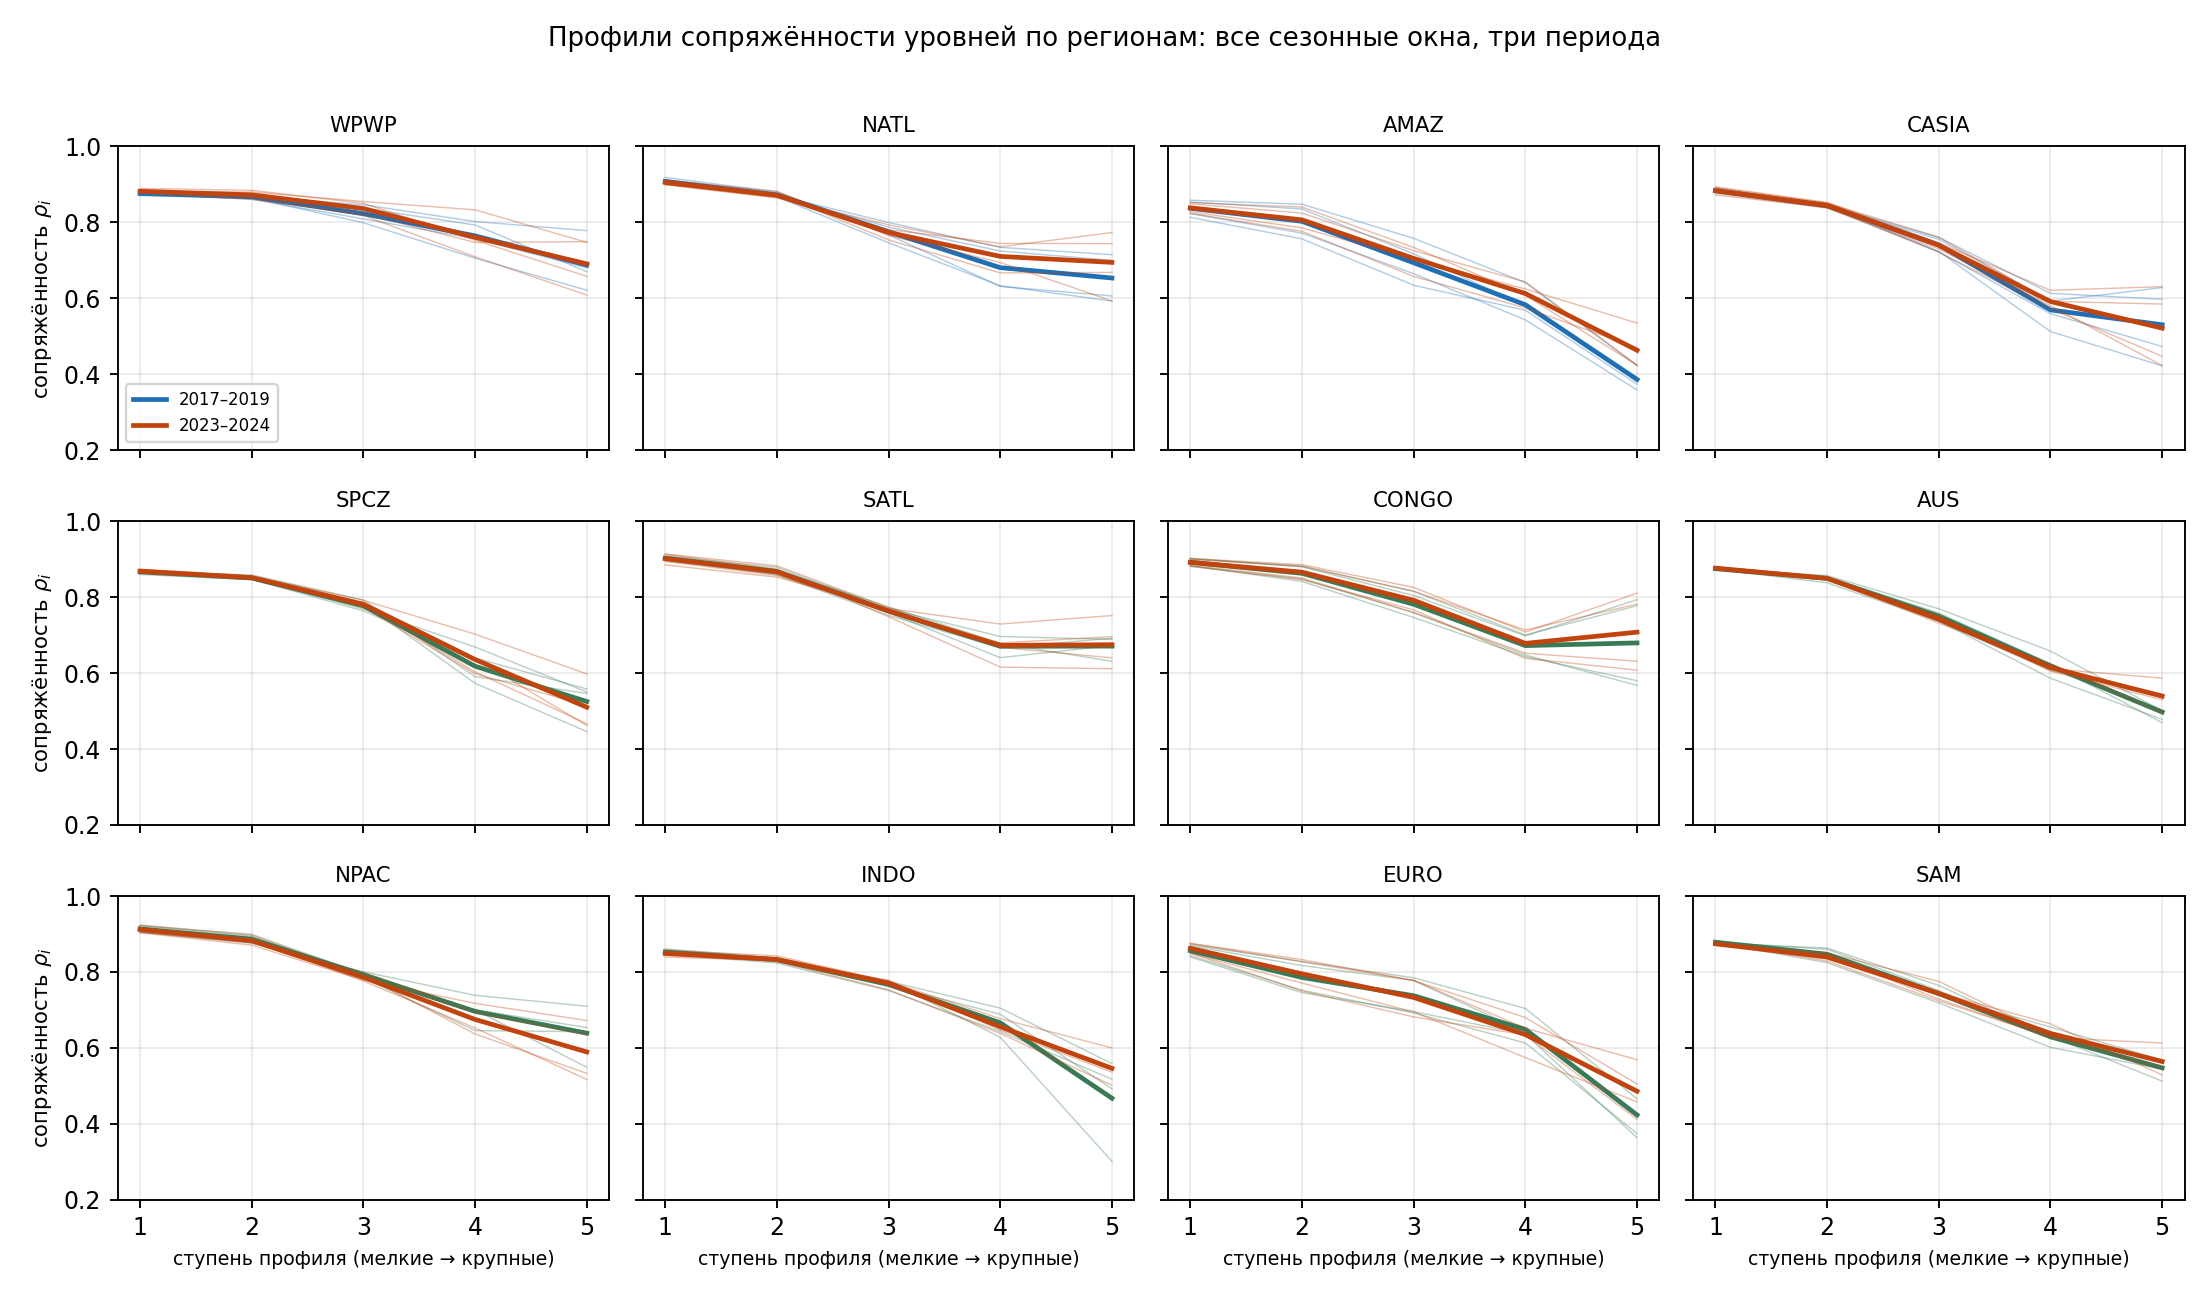
\includegraphics[width=\linewidth]{figures/figP_profiles.png}
\caption{Профили сопряжённости уровней $P$: тонкие линии --- отдельные сезонные окна, жирные --- средние по периодам 2017--2019, 2021--2022 и 2023--2024~гг. Ступени 1--5 отвечают парам соседних уровней: от (мельче~50; 50--100~км) до (400--800; 800--1600~км).}
\label{fig:profiles}
\end{figure}

\begin{figure}[t]
\centering
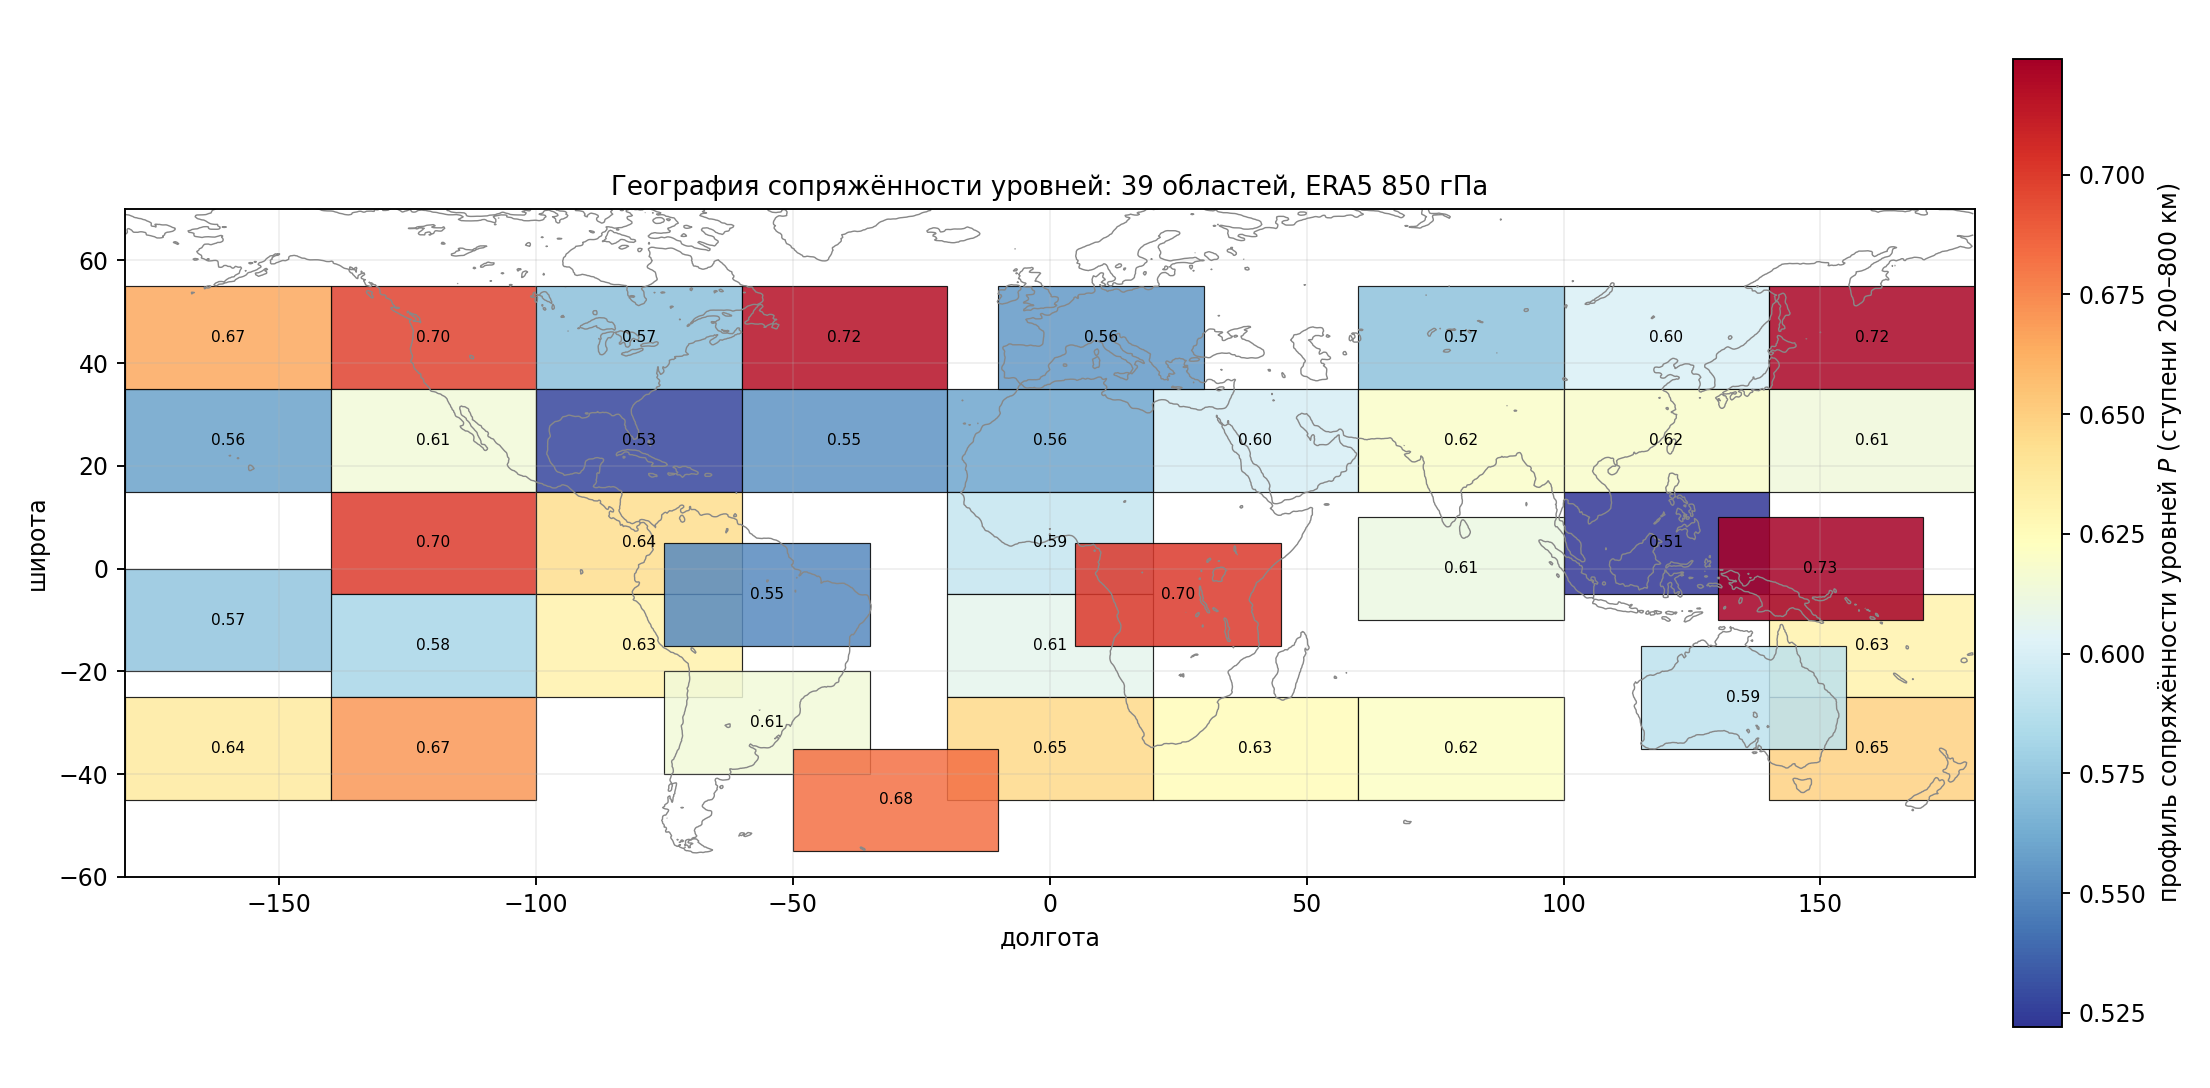
\includegraphics[width=\linewidth]{figures/figP_world_map.png}
\caption{География сопряжённости уровней: значения профиля на разрешённых ступенях (200--800~км) для 39 областей, ERA5, 850~гПа. Двенадцать областей выбраны содержательно, 27 --- формальным решёточным правилом.}
\label{fig:pmap}
\end{figure}

\subsection{Что выдерживают контроли}

Результаты проверок сведены в табл.~\ref{tab:tests}. Профиль образует устойчивую региональную сигнатуру на выборках, не участвовавших в его построении, не сводится к полуфрактальным характеристикам уровней и к скаттеринг-статистикам и воспроизводится в независимом реанализе. Одна оговорка приводится в явном виде: независимость профиля от полного спектра мощности носит условный характер --- она подтверждается при контроле спектральных признаков, но не выдерживает дополнительного контроля геометрии областей ($p=0{,}10$). Иными словами, часть межрегиональных различий профиля связана с широтой области и шагом сетки, и утверждение о полной несводимости к спектру мы не делаем.

\begin{table}[t]
\centering
\caption{Сводка проверок профиля сопряжённости. Приведены уровни значимости перестановочных тестов кластеризации (999 перестановок региональных меток); «независимые годы» --- выборки, не участвовавшие в построении дескриптора.}
\label{tab:tests}
\small
\begin{tabular}{@{}p{0.62\linewidth}p{0.30\linewidth}@{}}
\toprule
Проверка & Итог\\
\midrule
Региональная сигнатура, независимые годы и фазы ЭНСО & $p=0{,}001$\\
Сверх полуфрактальных характеристик уровней \cite{Krenke2019} & $p=0{,}001$\\
Сверх скаттеринг-статистик \cite{Cheng2024} & $p=0{,}026$\\
Сверх полного спектра мощности & $p=0{,}029$; с контролем геометрии $p=0{,}10$\\
Только разрешённые уровни (от 200~км) & $p=0{,}002$\\
Сигнатура в MERRA-2 & $p=0{,}001$\\
Согласие с расчётом по модели без усвоения наблюдений & $\rho=0{,}71$; $p=0{,}001$\\
\bottomrule
\end{tabular}
\end{table}

\subsection{Проверка по расчёту без усвоения наблюдений}

Согласие двух реанализов недостаточно для утверждения о свойстве атмосферы: ERA5 и MERRA-2 усваивают в основном одни и те же наблюдения, и совпадение их географии может отражать географию наблюдательной сети \cite{BonavitaLaloyaux2020}. Решающей проверкой служит расчёт по свободной модели, не усваивающей наблюдений вовсе.

Такое сопоставление выполнено (рис.~\ref{fig:free}). Региональная география сопряжённости в эксперименте \texttt{highresSST-present} воспроизводит географию ERA5 с ранговой корреляцией $\rho=0{,}71$ ($p=0{,}001$, 39 областей). Оценивать эту величину следует относительно внутреннего предела метода: корреляция между двумя независимыми периодами самого ERA5 составляет $0{,}93$, то есть достигнуто около трёх четвертей возможного. Различие естественно: свободный расчёт воспроизводит климатологию режимов, а не конкретную их реализацию.

Вывод существенен для всей постановки: измеряемое свойство относится к атмосфере, а не к системе наблюдений и не к системе усвоения. Ограничение, которое в работах такого рода обычно остаётся непреодолённым, здесь снято.

\begin{figure}[t]
\centering
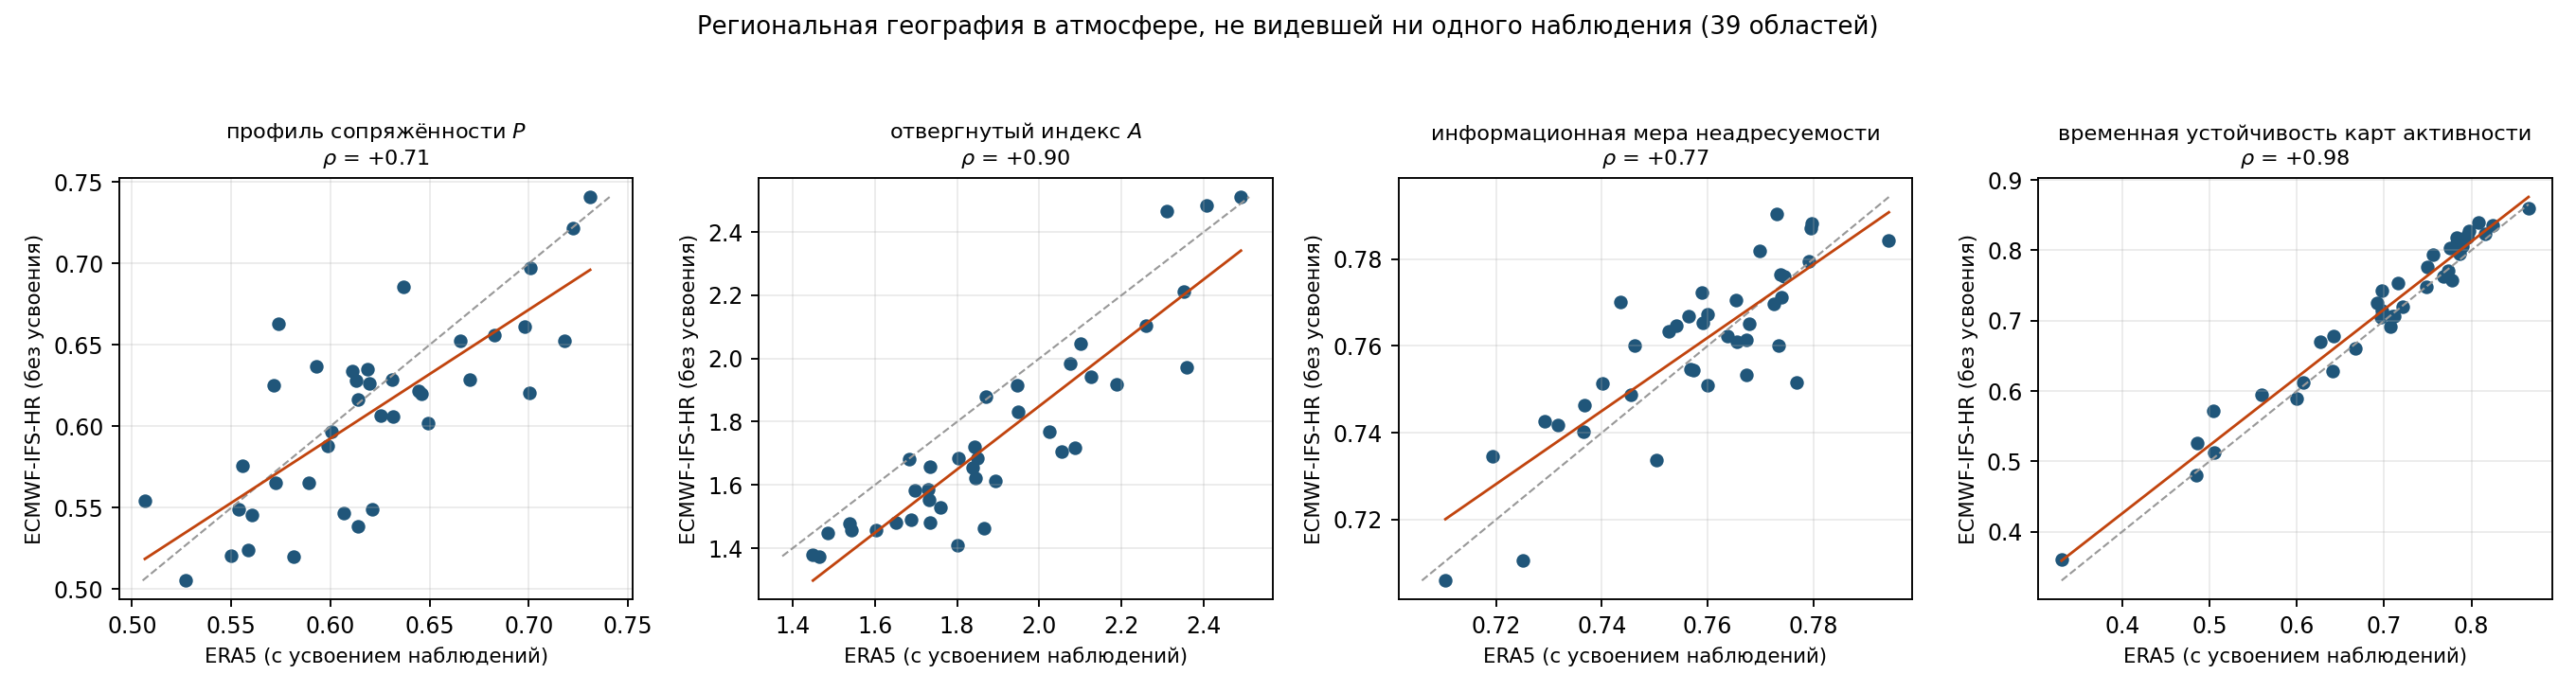
\includegraphics[width=\linewidth]{figures/figP_free_running.png}
\caption{Сопоставление региональной географии по ERA5 (ось абсцисс) и по свободному расчёту ECMWF-IFS-HR без усвоения наблюдений (ось ординат) для 39 областей. Слева направо: профиль сопряжённости $P$; отвергнутый индекс невзаимности $A$; информационная мера неадресуемости; временная устойчивость карт активности. Пунктир --- линия равенства.}
\label{fig:free}
\end{figure}

\subsection{Независимая проверка содержания величины}

Отдельно проверено, измеряет ли профиль то, что ему приписывается. Для этого построена независимая мера --- нормированная взаимная информация между картами активности соседних уровней, вычисляемая по рангам и потому нечувствительная к амплитуде поля. Профиль согласуется с ней с ранговой корреляцией $-0{,}93$ (величины по построению противоположны по знаку), при этом связь профиля с амплитудой полосы составляет лишь $+0{,}20$, а с временной устойчивостью карт активности --- $+0{,}02$.

Это не внешняя валидация: обе величины суть статистики одного совместного распределения, и высокая корреляция между ними означает согласованность, а не предсказательную силу. Но она устанавливает главное --- профиль является добросовестной сводкой именно той адресуемости, о которой идёт речь, и не является тенью ни амплитуды, ни инерции поля.

\subsection{Конго и Амазония}

Показательный случай --- два очага глубокой конвекции над сушей в близких широтах. При сходном режиме увлажнения бассейны Конго и Амазонии обнаруживают качественно различную архитектуру иерархии (рис.~\ref{fig:congo}). Различие сосредоточено на верхней ступени профиля: медиана по восьми сезонным окнам составляет $\rho_5=0{,}70$ для Конго против $0{,}42$ для Амазонии, тогда как на мелких ступенях профили близки (0,89 и 0,84 на первой ступени).

Содержательно это означает следующее. В бассейне Конго очаги мезомасштабной активности размещаются преимущественно там же, где активен соседний крупный уровень: совместное распределение рангов вытянуто вдоль диагонали, и по крупномасштабному полю можно указать, где окажется мезомасштаб. В Амазонии та же пара уровней распределена почти безразлично: мезомасштабная организация в значительной мере отвязана от крупного поля. Различие устойчиво по годам и воспроизводится на независимых периодах.

Пример показывает главное для приложений: дескриптор различает территории, неразличимые по стандартным характеристикам режима --- по количеству осадков, по конвективному потенциалу, по спектру, --- и различает их по признаку, прямо относящемуся к задаче генерализации. Именно в этом состоит его непосредственная польза для районирования.

\begin{figure}[t]
\centering
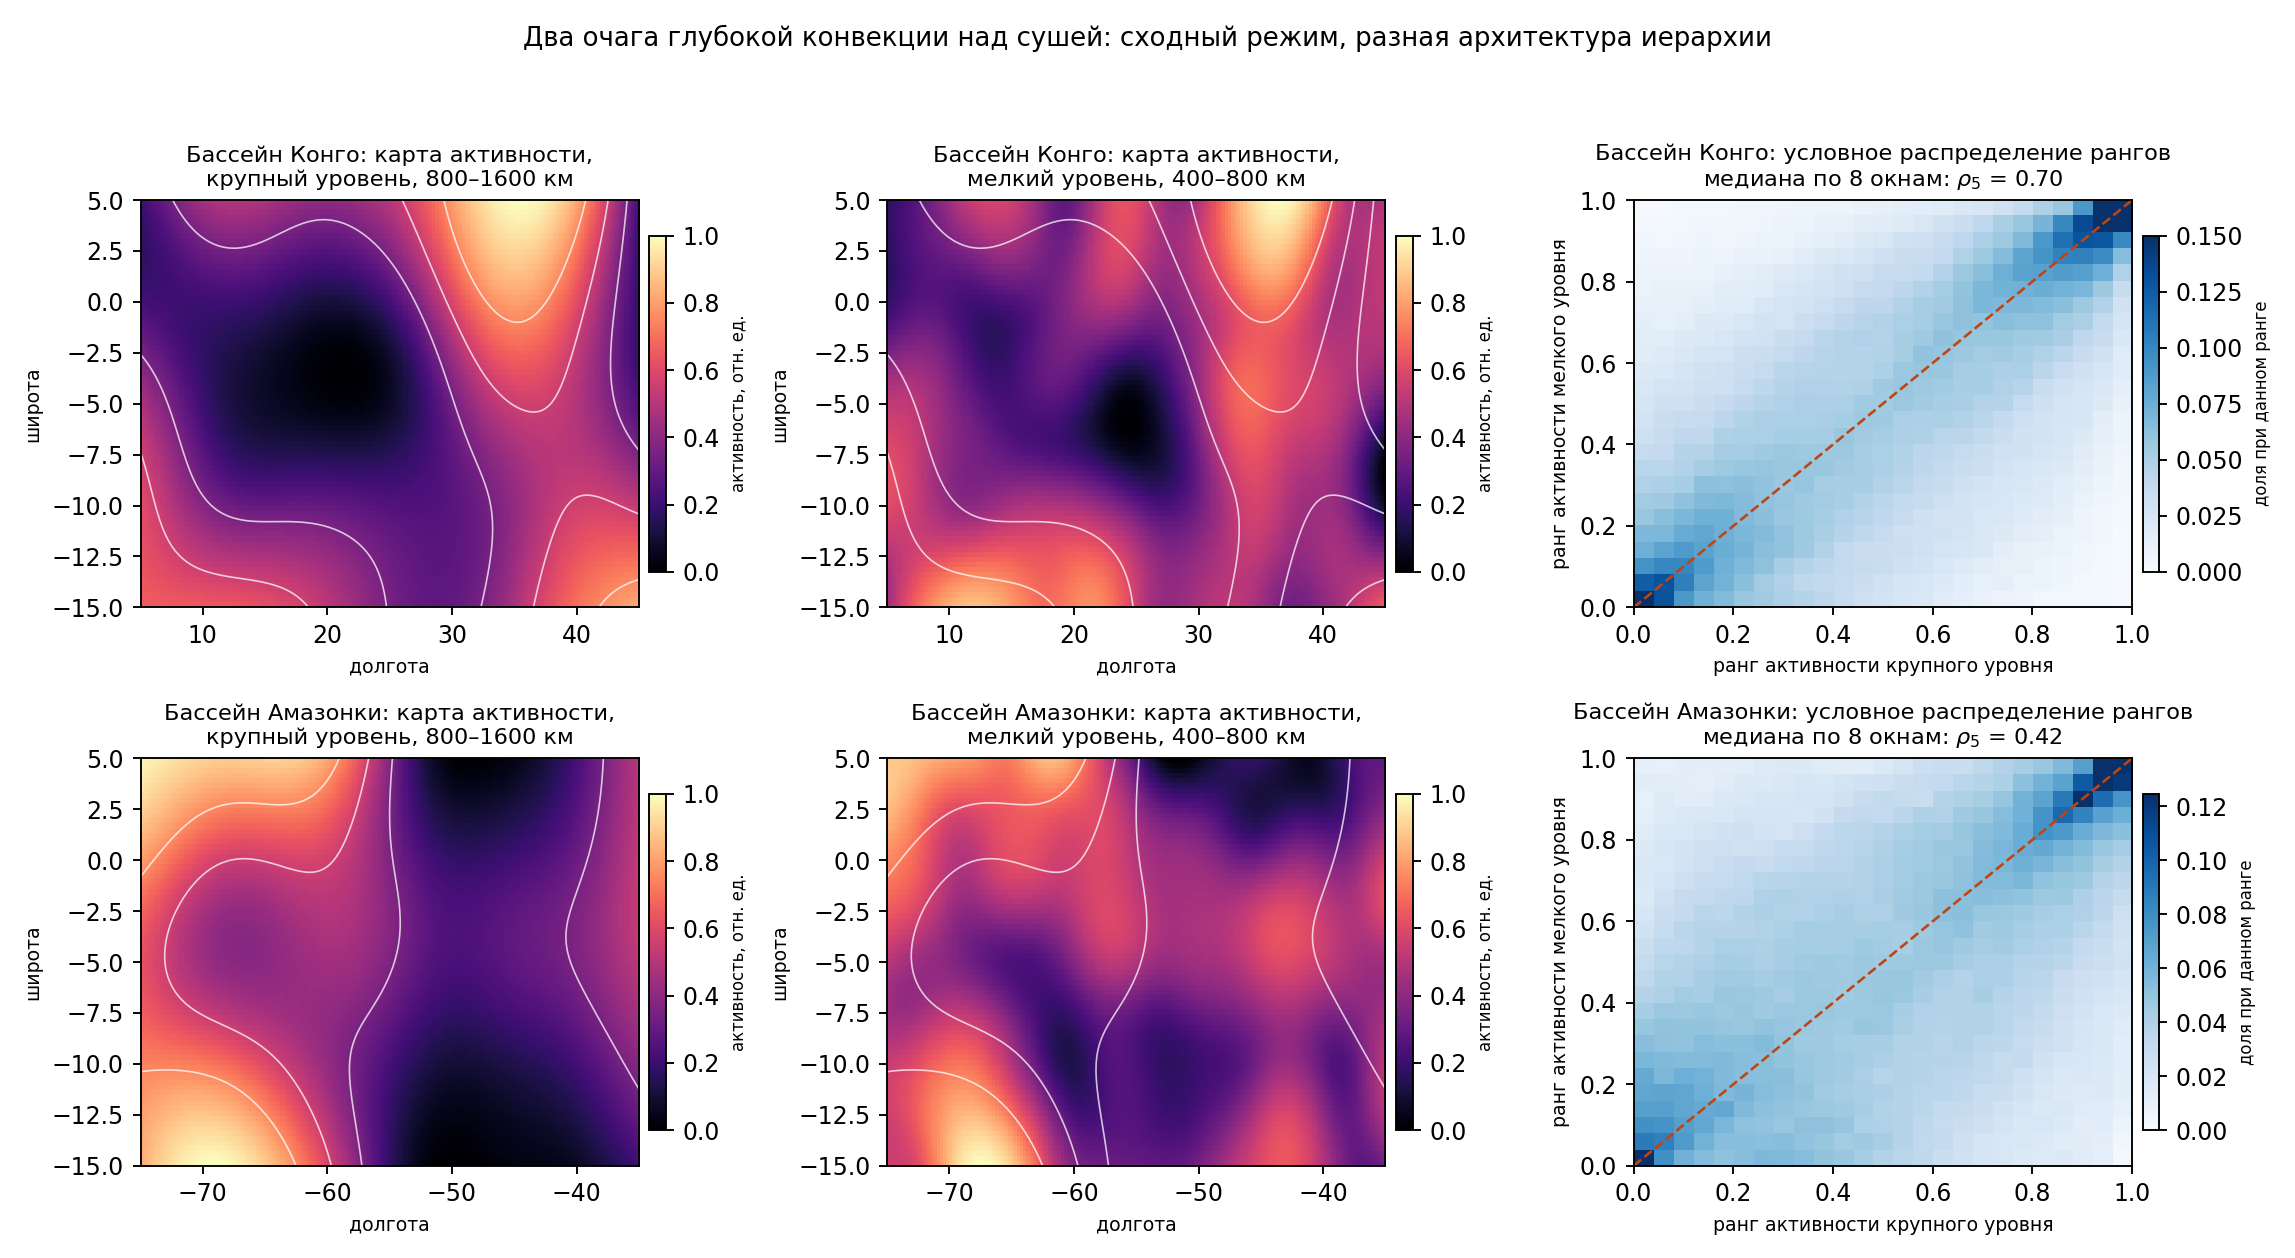
\includegraphics[width=\linewidth]{figures/figP_congo_amazon.png}
\caption{Бассейны Конго (вверху) и Амазонки (внизу), январь--март 2023~г. Слева и в центре --- карты активности крупного (800--1600~км) и мелкого (400--800~км) уровней на один срок; белые изолинии --- активность крупного уровня, одни и те же на обеих картах ряда. Справа --- совместное распределение пространственных рангов активности двух уровней по всем срокам окна; пунктир --- диагональ полного соответствия. В Конго мезомасштабная активность привязана к крупному полю, в Амазонии --- нет.}
\label{fig:congo}
\end{figure}

\section{Проверенные и отвергнутые интерпретации}
\label{sec:limits}

Наряду с подтверждёнными свойствами проверен и отвергнут ряд возможных истолкований. Мы приводим их полностью (табл.~\ref{tab:negative}): они очерчивают область корректного использования и предупреждают избыточное толкование.

\subsection{Отвергнутая конструкция второго дескриптора}

Первоначально наряду с профилем предлагался второй дескриптор --- индекс невзаимности $A$, построенный как мера того, насколько статистические операторы агрегирования и детализации не переставимы. Ему приписывался смысл необратимости географического обобщения: большие значения должны были означать, что размещение мезомасштаба не восстановимо по крупномасштабному полю даже статистически.

Индекс действительно образует устойчивую региональную сигнатуру, воспроизводится в MERRA-2 с $\rho=0{,}93$ и в свободном расчёте с $\rho=0{,}90$. Однако проверка содержания величины его не подтвердила. На синтетических полях, где восстановимость мелкого уровня по крупному задана по построению и планомерно меняется, индекс не реагирует на неё ни в пространственном прочтении ($\rho=-0{,}32$), ни в прочтении через предсказуемость коэффициентов уровней ($\rho=-0{,}35$), тогда как независимая информационная мера отзывается корректно ($+0{,}92$ и $-0{,}93$ соответственно). На тех же синтетических полях индекс монотонно и сильно следует за временн\'{о}й устойчивостью поля ($\rho=1{,}00$), и это подтверждается на реальных данных: связь индекса с устойчивостью карт активности составляет $+0{,}53$, а с информационной мерой неадресуемости --- $+0{,}03$. Более половины межрегиональной изменчивости индекса объясняется линейно набором из устойчивости, амплитуды, наклона спектра и геометрии области.

Заключение приходится сделать определённое: индекс $A$ --- воспроизводимая региональная характеристика атмосферы, но характеристика \emph{временн\'{о}й устойчивости} поля, а не необратимости обобщения. Приписанное ему истолкование отвергается; сама конструкция из основного изложения выводится. Причина ошибки установлена и носит методический характер: операторы оцениваются по скользящему окну, и чем медленнее меняется поле, тем систематичнее смещается результат.

\subsection{Прочие отвергнутые истолкования}

\emph{Дескрипторы не измеряют межмасштабный поток кинетической энергии.} Прямое сопоставление с потоком, вычисленным методом пространственного огрубления \cite{Germano1992,Aluie2018} на численном эксперименте с известным решением, объясняет доли процента его изменчивости против $0{,}35$--$0{,}47$ у стандартных характеристик поля деформации.

\emph{Простого закона, связывающего форму профилей со средовыми ковариатами, не обнаружено.} Ни перенормировка масштабной оси, ни очистка от зональной полосчатости, ни переход к полю интегрального переноса водяного пара не сводят профили разных регионов к единой кривой.

\emph{Вертикальной универсальности не обнаружено.} На уровне 500~гПа региональная сигнатура статистически не подтверждается, а согласие с географией уровня 850~гПа незначимо; объём выборки вдвое меньше основной, поэтому корректная формулировка --- отсутствие подтверждения, а не доказанное различие.

\emph{Информации о невязке влагобюджета дескрипторы не несут.} Невязка уравнения влагобюджета в реанализе определяется главным образом инкрементами усвоения \cite{Trenberth1991,Mayer2021}, и добавление межуровневых характеристик циркуляции к стандартному набору предикторов её описание не улучшает.

\emph{Мгновенной локальной связи с осадками нет.} На режимном уровне обнаруживается устойчивая отрицательная корреляция и запаздывающая структура с характерным временем около двух суток, согласующаяся с известным циклом расходования и восстановления конвективной энергии \cite{Masunaga2012,PetersNeelin2006}, однако формализовать это как динамическое уравнение не удалось, а характерное время частично воспроизводится инерцией самого оценивателя.

\begin{table}[t]
\centering
\caption{Проверенные и отвергнутые интерпретации.}
\label{tab:negative}
\small
\begin{tabular}{@{}p{0.56\linewidth}p{0.38\linewidth}@{}}
\toprule
Проверяемое положение & Итог проверки\\
\midrule
Индекс невзаимности $A$ измеряет необратимость обобщения & отвергнуто (не реагирует на управляемую восстановимость; следует за временн\'{о}й устойчивостью поля)\\
Дескрипторы отслеживают межмасштабный поток кинетической энергии & отвергнуто (характеристики поля деформации информативнее на два порядка)\\
Форма профилей подчиняется универсальному закону от средовых ковариат & отвергнуто (коллапса к единой кривой нет)\\
Дескрипторы вертикально универсальны (перенос на 500~гПа) & не подтверждено (уровнеспецифичность)\\
Дескрипторы информативны для замыкания влагобюджета реанализа & отвергнуто\\
Режимная связь с осадками формализуема как уравнение «источник--сток» & не установлено\\
Дескрипторы предсказывают скорость роста ошибки ансамблевого прогноза & отвергнуто (см. разд.~\ref{sec:applied})\\
Дескрипторы предсказывают уровень мезомасштабной ошибки анализа & отвергнуто (см. разд.~\ref{sec:applied})\\
\bottomrule
\end{tabular}
\end{table}

\section{Прикладное содержание: чем мы ограничены}
\label{sec:applied}

Естественное ожидание состоит в том, что мера подчинённости мезомасштаба крупному полю должна что-то говорить о качестве прогноза и о обоснованности статистической детализации. Это ожидание проверено на трёх независимых постановках, и ни одна не подтвердилась.

\emph{Скорость роста ошибки ансамблевого прогноза.} Сопоставление с оперативной ансамблевой системой на 39 областях не выявило связи предсказанного направления; более того, региональные различия скорости роста ошибки определяются бароклинностью --- связь с модулем широты составляет $+0{,}86$, --- а не архитектурой иерархии.

\emph{Уровень мезомасштабной ошибки в момент анализа.} Расхождение двух независимых систем усвоения на мезомасштабе, взятое как прямая мера неопределённости размещения, связано с дескрипторами лишь через амплитуду поля: после исключения контролей связь исчезает.

\emph{Потеря мезомасштаба в моделях машинного обучения.} Современные нейросетевые модели прогноза погоды \cite{Lam2023,Bi2023,Price2025} систематически теряют мезомасштабную изменчивость, и величина потери допускает точное измерение на общей платформе сопоставления \cite{Rasp2024}. На заблаговременности пять суток в полосе 200--800~км детерминированные модели теряют 55--69\,\% дисперсии, среднее по генеративному ансамблю --- 85\,\%, тогда как физическая модель и отдельная реализация генеративного ансамбля не теряют практически ничего. Механизм тем самым установлен однозначно: теряют те и только те системы, которые вычисляют условное среднее. Однако география этой потери и здесь предсказывается простой спектральной характеристикой лучше, чем предложенными дескрипторами.

Общий итог отрицателен, и его следует читать буквально. Мы располагаем данными, собираемыми наблюдательной сетью, чья плотность сама неоднородна географически, и моделями, которые --- в случае машинного обучения --- по устройству своих целевых функций уничтожают ровно ту мезомасштабную структуру, о которой идёт речь. В этих условиях отсутствие обнаруженной связи не позволяет заключить ни о наличии, ни об отсутствии прикладного содержания у измеренной величины. Оно позволяет заключить другое: на сегодняшних данных и сегодняшних моделях такое содержание не обнаруживается, а простая спектральная характеристика оказывается более сильным предиктором во всех трёх постановках. Дальнейшее продвижение требует не новых статистических проверок на том же материале, а иных наблюдений --- прежде всего однородных по плотности --- и моделей, сохраняющих мезомасштабную изменчивость.

\section{Выводы}
\label{sec:conclusion}

1.~Предложен компактный дескриптор межуровневой организации атмосферной циркуляции --- профиль сопряжённости октавных уровней $P$, характеризующий степень, в которой размещение мезомасштабной изменчивости предопределено соседним крупным уровнем.

2.~Дескриптор образует устойчивую региональную сигнатуру, сохраняющуюся при смене сезона, года и фазы ЭНСО ($p=0{,}001$ на выборках, не участвовавших в его построении), не сводится к полуфрактальным характеристикам уровней и к симметричным статистикам межмасштабной связи. Независимость от полного спектра мощности носит условный характер: она не выдерживает дополнительного контроля геометрии областей.

3.~Региональная география дескриптора воспроизводится не только в независимом реанализе, но и в модельном расчёте, не усваивающем никаких атмосферных наблюдений ($\rho=0{,}71$ при внутреннем пределе метода $0{,}93$). Измеряемое свойство относится к атмосфере, а не к наблюдательной сети и не к системе усвоения. Проверка содержания величины независимой информационной мерой подтверждает, что дескриптор измеряет именно адресуемость и не является тенью амплитуды или инерции поля.

4.~Наибольшая сопряжённость свойственна внетропическим штормовым путям, наименьшая --- влажно-конвективным океаническим режимам; бассейны Конго и Амазонии при сходном режиме обнаруживают качественно различную архитектуру иерархии. Полученная характеристика удовлетворяет операциональному определению инварианта динамики геосистем и продолжает линию исследований иерархической организации --- от выделения уровней к измерению их взаимодействия.

5.~Прикладное содержание величины на доступных сегодня данных и моделях не установлено. Три выведенных предсказания --- о скорости роста ошибки прогноза, об уровне мезомасштабной ошибки анализа и о потере мезомасштаба в моделях машинного обучения --- проверены и не подтвердились, причём во всех трёх случаях простая спектральная характеристика оказалась более сильным предиктором. Отрицательный результат воспроизводим и очерчивает направление дальнейшей работы: требуются наблюдения, однородные по плотности, и модели, сохраняющие мезомасштабную изменчивость.

6.~Первоначально предлагавшийся второй дескриптор --- индекс невзаимности операторов агрегирования и детализации --- сохраняет статус воспроизводимой региональной характеристики, но приписанное ему истолкование как меры необратимости обобщения отвергнуто прямой проверкой: величина следует за временн\'{о}й устойчивостью поля, а не за восстановимостью мезомасштаба.

\paragraph{Данные и код.} Протоколы проверок с заранее фиксированными критериями, программный код, полная таблица выполненных экспериментов и численные результаты открыты в репозитории: \url{https://github.com/Theclimateguy/Shroedinger}.

\printbibliography[title={Список литературы}]

\end{document}
